% $Header$

\documentclass[t,14pt,mathserif,xcolor=table]{beamer}

% This file is a solution template for:

% - Talk at a conference/colloquium.
% - Talk length is about 20min.
% - Style is ornate.



% Copyright 2004 by Till Tantau <tantau@users.sourceforge.net>.
%
% In principle, this file can be redistributed and/or modified under
% the terms of the GNU Public License, version 2.
%
% However, this file is supposed to be a template to be modified
% for your own needs. For this reason, if you use this file as a
% template and not specifically distribute it as part of a another
% package/program, I grant the extra permission to freely copy and
% modify this file as you see fit and even to delete this copyright
% notice. 


\input{style.tex}

\usepackage[brazil]{babel}
%\usepackage[english]{babel}

\usepackage{graphicx,url}	%Package para figuras
% or whatever

\usepackage[utf8]{inputenc}
% or whatever

\usepackage{times}
\usepackage[T1]{fontenc}
\usepackage{tabularx}
\usepackage{multirow}
\usepackage{adjustbox}
\usepackage{array}
%\usepackage[cmex10]{amsmath}
% Or whatever. Note that the encoding and the font should match. If T1
% does not look nice, try deleting the line with the fontenc.
\usepackage[linesnumbered,ruled,vlined]{algorithm2e}
\newcommand{\semitransp}[2][35]{\color{fg!#1}#2}

\title[] % (optional, use only with long paper titles)
{Encontrando os Top-K Influenciadores em uma Rede Social}

\subtitle{Vagner Clementino}

%\author[] % (optional, use only with lots of authors)
%{Vagner Clementino~\inst{1}} %\and S.~Another\inst{2}}
% - Give the names in the same order as the appear in the paper.
% - Use the \inst{?} command only if the authors have different
%   affiliation.

\institute[] % (optional, but mostly needed)
{
%  \inst{1}%
  Departamento de Ciência da Computação\\
  Universidade Federal de Minas Gerais(UFMG)\\
  Projeto e Análise de Algoritmos - 2015-1\\
  %\and
  %\inst{2}%
  %Department of Theoretical Philosophy\\
  %University of Elsewhere
  }
% - Use the \inst command only if there are several affiliations.
% - Keep it simple, no one is interested in your street address.

\date[2015/06/21] %o(optional, should be abbreviation of conference name)
%{Software Quality and Measurement 2015-1 \\Prof. Eduardo Figueiredo}
% - Either use conference name or its abbreviation.
% - Not really informative to the audience, more for people (including
%   yourself) who are reading the slides online

\subject{Projeto e Análise de Algoritmo}
% This is only inserted into the PDF information catalog. Can be left
% out. 



% If you have a file called "university-logo-filename.xxx", where xxx
% is a graphic format that can be processed by latex or pdflatex,
% resp., then you can add a logo as follows:

% \pgfdeclareimage[height=0.5cm]{university-logo}{university-logo-filename}
% \logo{\pgfuseimage{university-logo}}



% Delete this, if you do not want the table of contents to pop up at
% the beginning of each subsection:
\AtBeginSubsection[]
{
  \begin{frame}<beamer>{Outline}
    \tableofcontents[currentsection,currentsubsection]
  \end{frame}
}


% If you wish to uncover everything in a step-wise fashion, uncomment
% the following command: 

%\beamerdefaultoverlayspecification{<+->}

\expandafter\def\expandafter\insertshorttitle\expandafter{%
  \insertshorttitle\hfill%
  \insertframenumber\,/\,\inserttotalframenumber}

\setbeamertemplate{caption}[numbered]
\setbeamertemplate{bibliography item}{\insertbiblabel}
\begin{document}

\begin{frame}
  \titlepage
\end{frame}

\begin{frame}{Agenda}
  \tableofcontents
  % You might wish to add the option [pausesections]
\end{frame}


% Structuring a talk is a difficult task and the following structure
% may not be suitable. Here are some rules that apply for this
% solution: 

% - Exactly two or three sections (other than the summary).
% - At *most* three subsections per section.
% - Talk about 30s to 2min per frame. So there should be between about
%   15 and 30 frames, all told.

% - A conference audience is likely to know very little of what you
%   are going to talk about. So *simplify*!
% - In a 20min talk, getting the main ideas across is hard
%   enough. Leave out details, even if it means being less precise than
%   you think necessary.
% - If you omit details that are vital to the proof/implementation,
%   just say so once. Everybody will be happy with that.


\section{Contexto}

\begin{frame}{Contexto}
	\begin{itemize}
	
		\item Tradicionalmente as campanhas de marketing se baseiam em determinar um conjunto de consumidores, denominado público-alvo \cite{hughes1996complete}{}.
		
		\item A \textit{mineração de dados} permite a construção de modelos que tentam predizer o comportamento de um cliente baseado em seu histórico de compras \cite{kumar1999extracting}{}.
		
		\item  Nos casos em que esta abordagem têm sucesso, foi possível perceber um aumento na lucratividade \cite{piatetsky1999estimating}
		
		
		\end{itemize}
	
\end{frame}

%%%%%%%%%%%%%%%%%%%%%%%%%%%%%%%%%%%%%%%%%%%%%%%%%%%%%%%%%%%%%%%%%%%%%%%%%%%%%%%%%%%%%%%%%%%%%%%%%%%%%%555555

\begin{frame}{Contexto}

	\begin{itemize}
	
		\item O efeito que os demais consumidores possuem sobre a decisão de compra de um cliente é conhecido em Economia como \textit{externalidade da rede}{}. 
		
		\item Este \textit{``efeito da rede"} vêm crescendo em importância especialmente em setores ligados diretamente à informação (software, imprensa, telecomunicações e etc.) \cite{shapiro2013information}{}.
		
	\end{itemize}
	
\end{frame}
%%%%%%%%%%%%%%%%%%%%%%%%%%%%%%%%%%%%%%%%%%%%%%%%%%%%%%%%%%%%%%%%%%%%%%%%%%%%%%%%%%%%%%%%%%%%%%%%%%%%%%%%%%555

%%%%%%%%%%%%%%%%%%%%%%%%%%%%%%%%%%%%%%%%%%%%%%%%%%%%%%%%%%%%%%%%%%%%%%%%%%%%%%%%%%%%%%%%%%%%%%%%%%%%%%%%%%

\section{Problema}

\begin{frame}{Problema}

	\begin{itemize}
	
		\item Suponha uma empresa de marketing digital que pretende divulgar um novo produto \emph{A} da marca  para o maior número possível de usuários em determinada rede social.
		
		\item Possíveis estratégias:
			\begin{itemize}
				\item \textit{Marketing de Massa}
				\item \textit{Marketing Direcionado}
				\item \textbf{Divulgar para usuários que possam ``influenciar" os demais}
			\end{itemize}
		
	\end{itemize}
	
\end{frame}

%%%%%%%%%%%%%%%%%%%%%%%%%%%%%%%%%%%%%%%%%%%%%%%%%%%%%%%%%%%%%%%%%%%%%%%%%%%%%%%%%%%%%%%%%%%%%%%%%%%%

\begin{frame}{O Problema Máxima Influência}

	\begin{itemize}
		\item Dado grafo não direcionado $G(V,E)${}
			\begin{itemize}
				\item $V$ representa os possíveis consumidores
				\item $E$ representam os relacionamentos sociais entre consumidores		
			\end{itemize}
			
		\item Encontrar $W \subset V${}, de modo que $\left\vert W \right\vert\leq K$ e $\cup_{j=1}^{k} w_{j}$ é \textit{maximizado}
		\item Onde $w_j$ tal que $ 1 \leq j \leq k$ é alguma função sobre os vértices em $V$
		\item No contexto deste trabalho, maximizar $\cup_{j=1}^{k} w_{j}$ significa \textit{``influenciar" a compra de um produto por um conjunto maior de usuários}{}
	
		
	\end{itemize}
	
\end{frame}
%%%%%%%%%%%%%%%%%%%%%%%%%%%%%%%%%%%%%%%%%%%%%%%%%%%%%%%%%%%%%%%%%%%%%%%%%%%%%%%%%%%%%%%%%%%%%%%%%%%%%%%%

\begin{frame}{O Problema Máxima Influência}

	\begin{itemize}
		\item  0 problema de determinar um valor de $k$ que maximize a influência é NP-Difícil \cite{Garey:1979:CIG:578533}{}
	   \item Existe na literatura um algoritmo guloso que consegue um fator de aproximação da ordem de $1-\frac{1}{e}$ (aproximadamente 63\%) \cite{Hochbaum:1996:ACP:241938.241941}
	  \item  Algoritmo baseado na abordagem apresentada em \cite{domingos2001mining}.
		
	\end{itemize}
	
\end{frame}
%%%%%%%%%%%%%%%%%%%%%%%%%%%%%%%%%%%%%%%%%%%%%%%%%%%%%%%%%%%%%%%%%%%%%%%%%%%%%%%%%%%%%%%%%%%%%%%%%%%%%%%%

%%%%%%%%%%%%%%%%%%%%%%%%%%%%%%%%%%%%%%%%%%%%%%%%%%%%%%%%%%%%%%%%%%%%%%%%%%%%%%%%%%%%%%%%%%%%%%%%%%%%%%
\section{Objetivo}

\begin{frame}{Objetivo}

	\begin{itemize}
		\item Propor uma heurística que encontre $W \subset V${} tal que $\left\vert W \right\vert\leq K$ de modo a maximizar o número de usuários influenciados na rede.
		
		\item A Heurística é baseada na \textit{Cobertura de Vértice} \cite{Cormen:2009:IAT:1614191}{}.
		
	\end{itemize}
	
\end{frame}

%%%%%%%%%%%%%%%%%%%%%%%%%%%%%%%%%%%%%%%%%%%%%%%%%%%%%%%%%%%%%%%%%%%%%%%%%%%%%%%%%%%%%%%%%%%%%%%%%%%%%%%%
\section{Modelo Proposto}

\begin{frame}{Cobertura de Vértices}

	\begin{itemize}
		\item Dado um grafo $G=(V,E)$ e um número inteiro $K\leq\left\vert V\right\vert$.
		\item Existe um subconjunto $V^{'} \subseteq V$ tal que $\left\vert V '\right\vert\leq K$ tal que cada vértice $\left\{ u,v\right\} \in E$, pelo menos um, $u$ ou $v$, pertence a $V^{'}${}.	
		\item Problema \textit{NP-completo}{} \cite{Garey:1979:CIG:578533, Cormen:2009:IAT:1614191}{}.
		\item Existe um algoritmo aproximado com nível de aproximação igual a \textit{2}.
	\end{itemize}
	
\begin{figure}[!t]
	\centering
	\includegraphics[width=.7in]{../img/vertex_cover.png}
	\label{fig_vertex_cover}
	\caption{Cobertura de Vértice}
\end{figure}
	
\end{frame}

%%%%%%%%%%%%%%%%%%%%%%%%%%%%%%%%%%%%%%%%%%%%%%%%%%%%%%%%%%%%%%%%%%%%%%%%%%%%%%%%%%%%%%%%%%%%%%%%%%%%%%%%%%%%%

\begin{frame}{Heurística Proposta}

	\begin{itemize}
		\item  Seja $A_0 \in V$ e $|A_0| \leq k$ e $A_0$ maximize o número de usuários influenciados
		\item  Seja $C \in V$ a cobertura de vértice de um $G(V,E)$ obtida utilizando a heurística proposta em \cite{Cormen:2009:IAT:1614191}.
		\item $C$ é no máximo $ 2 \times C^{*}$, onde $C^{*}$ é a Cobertura de Vértice ótima para o grafo $G(V,E)$.
		\item $v \in C$ é um bom candidato para estar em $A_0$.
		
	\end{itemize}
	

	
\end{frame}

%%%%%%%%%%%%%%%%%%%%%%%%%%%%%%%%%%%%%%%%%%%%%%%%%%%%%%%%%%%%%%%%%%%%%%%%%%%%%%%%%%%%%%%%%%%%%%%%%%%%%%%%%%%%%

\begin{frame}{Heurística Proposta}

	\begin{itemize}
		\item Na prática $C \gg k$, logo devemos escolher os ``melhores"{} vértice em $C$
		\item Caso $|C| = k$ podemos naturalmente definir $A_{0} = C$.
		\item Do contrário, devemos encontrar no máximo $k$ vértice em $C$ para fazer parte de $A_{0}$.
		\item Escolha gulosa baseada na métrica \textsc{DEGREE ACESSS}{}
	\end{itemize}
	
\end{frame}

%%%%%%%%%%%%%%%%%%%%%%%%%%%%%%%%%%%%%%%%%%%%%%%%%%%%%%%%%%%%%%%%%%%%%%%%%%%%%%%%%%%%%%%%%%%%%%%%%%%%%%%%%%%%%

\begin{frame}[shrink=50]{Algoritmo Proposto}

\begin{algorithm}[H]
\DontPrintSemicolon % Some LaTeX compilers require you to use \dontprintsemicolon instead
\SetKwFunction{FINVERTEXCOVER}{FIND-VERTEX-COVER}
\SetKwFunction{CALCULEDEGREEACESSS}{CALCULE-DEGREE-ACESSS}
\SetKwFunction{SORT}{SORT}
\SetKwFunction{DEQUEUE}{DEQUEUE}
\KwIn{Um grafo não direcionado e não ponderado $G(V,E)$\\
	  um inteiro $k$ correspondente a primeiro índice de $A$;\\
	  um inteiro $r$ correspondente ao último índice de $A$}
\KwOut{Um conjunto $A_{0} \in V$ tal que $ 1 \leq |A_{0}| \leq k$}
	
	$C \gets \emptyset$\;
	$A_{0} \gets \emptyset$\;
	$Q \gets \emptyset$ {$Q$ é uma fila}\;
	
	$C \gets $ \FINVERTEXCOVER{$G(V,E)$}\;
	\If{$|C| = k$}{
		
		$A_{0} \gets C$\;
		\Return{$A_{0}$}\;	
	
	}\Else{
	
		\CALCULEDEGREEACESSS{$G(V,E),C$}\;
		\SORT{$C$} {Ordenando o conjunto $C$ em ordem decrescente ao grau acessibilidade.}\;
		$Q \gets C${Atribuindo o conjunto $C$ para uma fila}\;
		\While{$|A| < k$ \textbf{or} $Q$ \textbf{is not} $\emptyset$} {
			
			$v \gets $ \DEQUEUE{$Q$}\;
			
			\If{$v.degreeAcess > 0$}{
			
				$A_{0} \gets A_{0} \cup v$\;
			
			}
			
		
		}
		\Return{$A_{0}$}\;		
	
	}
\Return{$A_{0}$}\;
\caption{{\sc FIND-SEEDS} retorna o conjunto semente $A_0$ com base na Cobertura de Vértice de um grafo.}
\label{algo:define_sementes}
\end{algorithm}

\end{frame}
%%%%%%%%%%%%%%%%%%%%%%%%%%%%%%%%%%%%%%%%%%%%%%%%%%%%%%%%%%%%%%%%%%%%%%%%%%%%%%%%%%%%%%%%%%%%%%%%%%%%%%%%%%%%%

\begin{frame}{Análise do Algoritmo}

	\begin{itemize}
		\item O método \textsc{CALCULE-DEGREE-ACESSS}{} calcula o número de vértices que podem ser alcançados a partir de um vértice $v$
		\begin{itemize}
		
			\item Baseado no \textit{BFS}{}.
			\item \textit{Complexidade de Tempo} $O(V+A)${}.
			\item Executado $|C|$ vezes{}.
		
		\end{itemize}

		\item No pior caso $|C| = |V|$, complexidade do Algoritmo é dada por $O(V^{2}+VA)${}.
		
		\item \textit{Complexidade de Espaço} $O(V+A)$ (lista de adjacência){}.
		
	\end{itemize}




\end{frame}

%%%%%%%%%%%%%%%%%%%%%%%%%%%%%%%%%%%%%%%%%%%%%%%%%%%%%%%%%%%%%%%%%%%%%%%%%%%%%%%%%%%%%%%%%%%%%%%%%%%%%%%%

\section{Avaliação}

\begin{frame}{Avaliação}

	\begin{itemize}
		
		\item Baseada em \textit{Modelo de Propagação}
		\item Utilizada o modelo conhecido como \textit{Linear Threshold Model} \cite{granovetter1978threshold, schelling2006micromotives}{}
		\begin{itemize}
			\item Cada vértice $v$ recebe um valor aleatório $\theta_v$
			\item  $v$ é influenciado por cada um dos seus vizinhos $w$ de acordo com um peso $b_{v,w}$ que respeita a Equação \ref{eq:pesos_vizinhos}{}.
		\end{itemize}	
		
	\end{itemize}
	
\begin{equation} \label{eq:pesos_vizinhos}
\sum\limits_{\textrm{w vizinho de v}}{b_{v,w} \leq 1}
\end{equation}


\end{frame}
%%%%%%%%%%%%%%%%%%%%%%%%%%%%%%%%%%%%%%%%%%%%%%%%%%%%%%%%%%%%%%%%%%%%%%%%%%%%%%%%%%%%%%%%%%%%%%%%%%%%%%%%

\begin{frame}{Avaliação}

	\begin{itemize}
		
		\item $v$ se torna \textit{ativo} se o somatório dos pesos de seus vizinhos \textit{ativos} sejam $\geq \theta_v$, conforme Equação \ref{eq:ativacao}{}
		
		\item Baseline  \cite{kempe2003maximizing} 
		
	\begin{itemize}
		\item Algoritmo guloso
		\item Na primeira abordagem os vértices em $A_{0}$ foram escolhidas randomicamente;
		\item Na segunda heurística, foram escolhidos $k$ vértices em ordem decrescente de seu grau $d_{v}$;
		\item A terceira abordagem utilizou o conceito de \textit{Distance centrality} \cite{scott2012social}
	\end{itemize}
		
		
	\end{itemize}
	
\begin{equation} \label{eq:ativacao}
\sum\limits_{\textrm{w é um vizinho ativo de v}}{b_{v,w} \geq \theta_v}
\end{equation}

\end{frame}
%%%%%%%%%%%%%%%%%%%%%%%%%%%%%%%%%%%%%%%%%%%%%%%%%%%%%%%%%%%%%%%%%%%%%%%%%%%%%%%%%%%%%%%%%%%%%%%%%%%%%%%%

\begin{frame}{Dataset}

	\begin{itemize}
		
		\item Grafo de colaboração obtido a partir de coautorias em publicações de física\cite{snapnets}.
		\item Redes de coautoria são capazes de capturar as principais características das redes sociais de modo mais geral \cite{newman2001structure}.
	\item O gráfico de colaboração contém um vértice para cada pesquisador com artigo em \textit{arXiv}\footnote{\url{http://arxiv.org/}}
	\begin{itemize}	
		\item 9877 Vértices
		\item 51971 Aresta	
	\end{itemize}
	
	\end{itemize}
\end{frame}
%%%%%%%%%%%%%%%%%%%%%%%%%%%%%%%%%%%%%%%%%%%%%%%%%%%%%%%%%%%%%%%%%%%%%%%%%%%%%%%%%%%%%%%%%%%%%%%%%%%%%%%%
\section{Resultados}

\begin{frame}{Resultados}

\begin{table}[h]
\centering
\resizebox{\textwidth}{!}{%
\begin{tabular}{|l|c|c|c|c|c|}
\hline
\rowcolor[HTML]{C0C0C0} 
\multicolumn{1}{|c|}{\cellcolor[HTML]{C0C0C0}{\color[HTML]{000000} {\bf |V|}}} & {\color[HTML]{000000} {\bf k}} & {\color[HTML]{000000} {\bf |C|}} & {\color[HTML]{000000} {\bf |C| / |V|}} & \multicolumn{1}{l|}{\cellcolor[HTML]{C0C0C0}{\bf Vértices Ativos}} & {\color[HTML]{000000} {\bf \% Vértices Ativos}} \\ \hline
 & 5 & 8438 & 0,8543 & 2173 & 0,22 \\ \cline{2-6} 
 & 10 & 8438 & 0,8543 & 2173 & 0,22 \\ \cline{2-6} 
 & 15 & 8435 & 0,8540 & 2469 & 0,25 \\ \cline{2-6} 
 & 20 & 8433 & 0,8538 & 2766 & 0,28 \\ \cline{2-6} 
 & 25 & 8438 & 0,8543 & 2963 & 0,30 \\ \cline{2-6} 
\multirow{-6}{*}{9877} & 30 & 8435 & 0,8540 & 2963 & 0,30 \\ \hline
\end{tabular}
}
\caption{Resultados para diversos valores de k}
\label{tab:results}
\end{table}



	
\end{frame}
%%%%%%%%%%%%%%%%%%%%%%%%%%%%%%%%%%%%%%%%%%%%%%%%%%%%%%%%%%%%%%%%%%%%%%%%%%%%%%%%%%%%%%%%%%%%%%%%%%%%%%%%

\begin{frame}{Resultados}

\begin{figure}[!t]
	\centering
	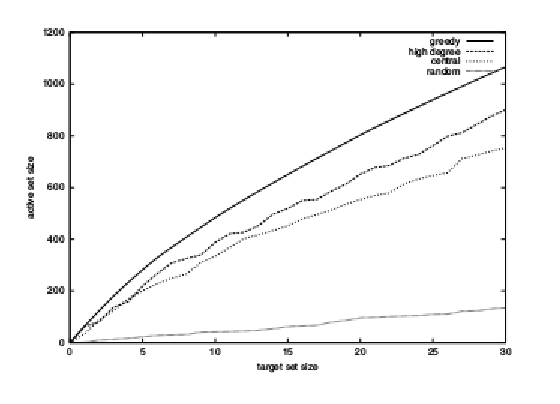
\includegraphics[width=2.0in]{../img/grafico_baseline.eps}
	\label{fig_vertex_cover}
	
\end{figure}


\begin{figure}[!t]
	\centering
	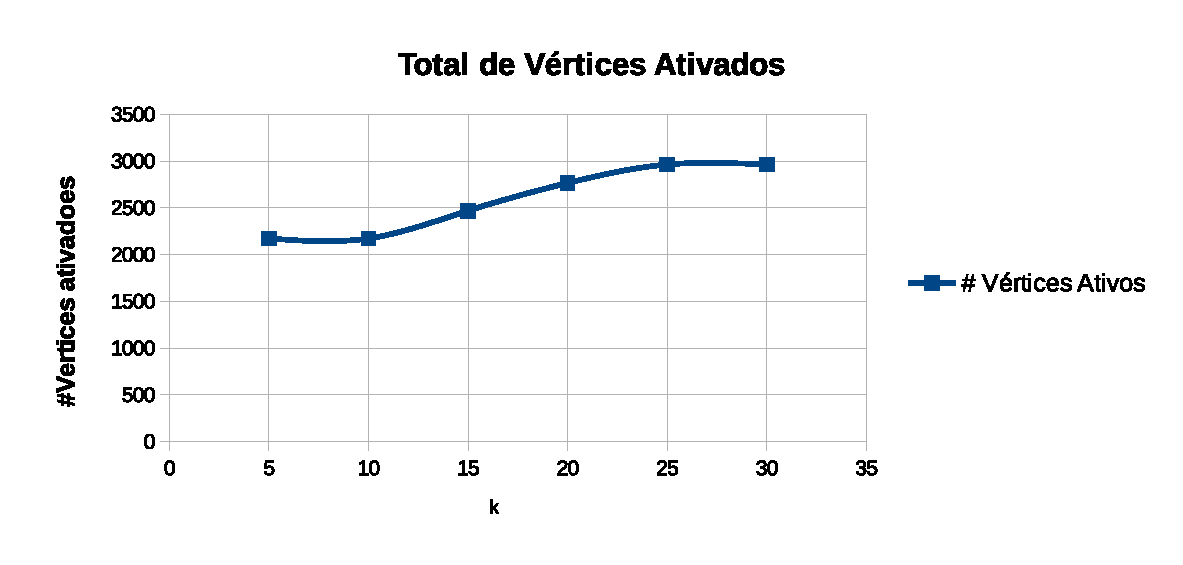
\includegraphics[width=2.5in]{../img/grafico_total.eps}
	\label{fig_vertex_cover}

\end{figure}


\end{frame}

%%%%%%%%%%%%%%%%%%%%%%%%%%%%%%%%%%%%%%%%%%%%%%%%%%%%%%%%%%%%%%%%%%%%%%%%%%%%%%%%%%%%%%%%%%%%%%%%%
\begin{frame}{Resultados}

	\begin{itemize}
		
		\item Resultados da heurística melhor em média, mesmo para valor de $k$ menores
		\item Variação do total de vértices ativados não acompanha o valor de $k$
		\item Valor de $k= 25$ se mostrou o ideal.
		\item Resultados bem abaixo da melhor solução \cite{Hochbaum:1996:ACP:241938.241941} 		
		
	\end{itemize}	


\end{frame}

%%%%%%%%%%%%%%%%%%%%%%%%%%%%%%%%%%%%%%%%%%%%%%%%%%%%%%%%%%%%%%%%%%%%%%%%%%%%%%%%%%%%%%%%%%%%%%%%%%%%

\section{Ameaças à Validade}

\begin{frame}{Ameaças à Validade}

	\begin{itemize}
		
		\item Modelo de Propagação é artificial
		\item A métrica \textsc{DEGREE ACESSS}{} não foi validada.
		\item Modelo aplicado a um único grafo.
		\item A escalabilidade da heurística não foi testada.		
	\end{itemize}	


\end{frame}




\section{Conclusões e Trabalhos Futuros}

\begin{frame}{Conclusões e Trabalhos Futuros}

	\begin{itemize}
		
		\item Heurística alcançou resultados satisfatórios.
		\item Heurística proposta possibilita refinamentos.
		\item Aplicação em grafos reais.
		\item Utilização de outros característica das redes sociais para a escolha gulosa.			
		
	\end{itemize}	


\end{frame}


\begin{frame}[allowframebreaks]
   \frametitle{References}
   \bibliographystyle{IEEEtranS}
   \bibliography{IEEEfull,bibliografia}
\end{frame}

\end{document}
